
\documentclass[tikz,convert={convertexe={magick.exe}}]{standalone}

\begin{document}
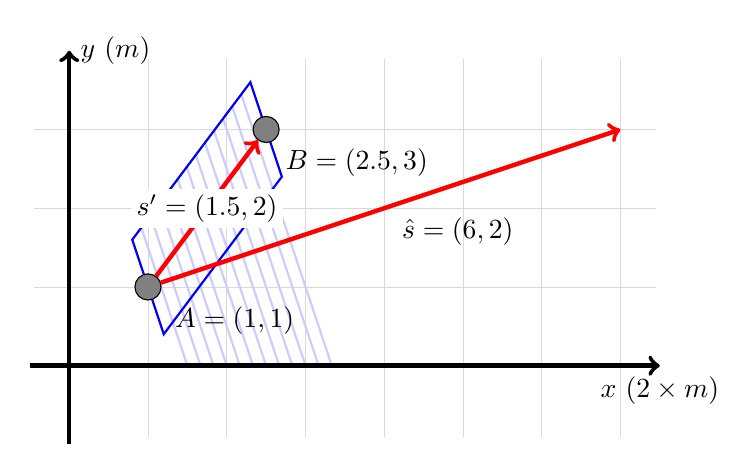
\begin{tikzpicture}[xscale=.5]
\draw[help lines, color=gray!30] (-.9,-.9) grid[xstep=2] (14.9,3.9);
\foreach \x in {1,...,12} {
	\coordinate (up) at (1.6+\x*3/13,1.6+\x*2/13) {};
	\coordinate (down) at (2.4+\x*3/13,.4+\x*2/13) {};
	\draw[draw=blue!20, thick] (up) --
	(intersection cs: first line={(up)--(down)}, second line = {(0,0)--(1,0)});
}
\draw[draw=blue, thick] (1.6,1.6) -- (2.4,.4) -- (5.4,2.4) -- (4.6,3.6) -- cycle;

\node (A) at (2,1) [circle, draw, fill=gray, label=below right:{$\;A = (1,1)$}] {};
\node (B) at (5,3) [circle, draw, fill=gray, label=below right:{$B = (2.5,3)$}] {};


\draw[->, ultra thick] (-1,0)--(15,0) node[below]{$x$ ($2 \times m$)};
\draw[->, ultra thick] (0,-1)--(0,4) node[right]{$y$ ($m$)};

\draw[->, ultra thick, red] (A) -- (14,3)
	node[midway, below right, black]{$\hat s = (6,2)$};
\draw[->, ultra thick, red] (A) -- (B)
	node[midway, fill=white, text=black, inner sep = .2em]{$s' = (1.5,2)$};
\end{tikzpicture}
\end{document}